\documentclass{beamer}
\usetheme{fibeamer}
\usepackage[main=english,portuguese]{babel}
\selectlanguage{portuguese}

\usepackage{csquotes}
\usepackage{graphicx}
\usepackage{multicol}

\graphicspath{{img/}}

\title{Curso de Desenvolvimento GBA}
\subtitle{1. Introdução ao GBA}
\author{João Paulo Taylor Ienczak Zanette}

\begin{document}

\maketitle

\begin{darkframes}
    \begin{frame}{Índice}
        \tableofcontents
    \end{frame}

    \section{Introdução}
    \subsection{Contextualização do Curso}

    \begin{frame}{Objetivos}
        \begin{itemize}
            \item Ensinar programação de baixo-nível (comunicação direta com
                hardware/integração com assembly);
            \item Ensinar técnicas de programação aplicadas;
            \item Mostrar o funcionamento de imagens/gráficos e áudio no mundo
                digital;
            \item Relacionar as tecnologias vistas com as utilizadas
                atualmente.
        \end{itemize}
    \end{frame}

    \begin{frame}{Programação}
        \begin{itemize}
            \item Assembly ARM7-TDMI --- Modo Thumb (GBA);
            \item OpenGL (NDS);
            \item C++ (GBA/NDS).
        \end{itemize}

        A mesma forma de programação para GBA serve também para: GB, GBC, NES,
        SNES, MegaDrive, SegaSaturn e PSX (PS1).
    \end{frame}

    \begin{frame}{Circuitos e Técnicas Digitais}
        \begin{itemize}
            \item Leitura/escrita de registradores (em que cada bit é mapeado
                para uma função específica) via programação;
        \end{itemize}
    \end{frame}

    \begin{frame}{Sistemas Digitais}
        \begin{itemize}
            \item Compreensão a respeito de como o Assembly gerado pela
                compilação altera o estado/memória do circuito;
            \item Compreensão do sistema que gera imagens em um circuito
                digital (VGA, LCD, etc\ldots);
            \item Funcionamento (inclusive a nível de circuito) da execução de
                músicas em formato de instrução MIDI\@;
            \item Técnicas de otimização através de Hardware.
        \end{itemize}
    \end{frame}

    \begin{frame}{Computação Gráfica}
        \begin{itemize}
            \item Desenho de primitivas (linhas, triângulos, circuitos, etc\ldots);
            \item Aceleração gráfica via Hardware.
        \end{itemize}
    \end{frame}

    \begin{frame}{Notações}
        \begin{center}
            \begin{tabular}{r|l}
                \texttt{0b???}      & \enquote{???} está em binário (\texttt{0b11111111 = 255}).\\
                \texttt{0x???}      & \enquote{???} está em hexadecimal (\texttt{0xFF = 255}).\\
                \texttt{???b}       & \enquote{???} está em binário (\texttt{11111111b = 255}).\\
                \texttt{???h}       & \enquote{???} está em hexadecimal (\texttt{FFh = 255}).\\
                \texttt{????:????}  & \enquote{:} serve apenas para melhor visualização \\
                                    & (\texttt{0x04000000 = 0400:0000h}).\\
                \texttt{??? $>>$ x} & \enquote{???} deslocado "x"\ bits para direita.\\
                \texttt{??? $<<$ x} & \enquote{???} deslocado "x"\ bits para esquerda.\\
            \end{tabular}
        \end{center}
    \end{frame}


    \subsection{Evolução dos consoles}
    \begin{frame}{Hello, World!}
        \begin{multicols}{2}
            Um breve prólogo das especificações técnicas e limitações dos consoles de
            VideoGame ao longo do tempo e uma análise de sua evolução.
            \begin{figure}[h!]
                \centering
                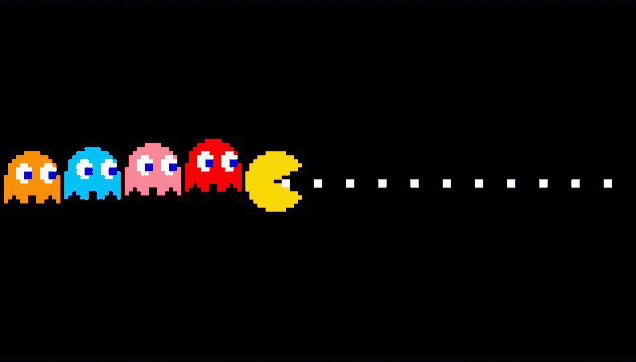
\includegraphics[width=.5\textwidth]{pacman}
            \end{figure}
        \end{multicols}
    \end{frame}

    \begin{frame}{Atari 2600 (1977)}
        \begin{multicols}{2}
            \begin{description}
                \item[Processador:] MOS Technology 6507 (variante do 6502 de 1975)
                \item[Barramento:] 8 bits
                \item[Clock:] 1.19MHz
                \item[RAM:] 128 bytes
                \item[ROM:] 16KB
                \item[Resolução:]
                    \begin{itemize}
                        \item 160x192 (NTSC)
                        \item 160x228 (PAL)
                    \end{itemize}
                \item[Cores:] 128
                \item[Som:] 2 canais (1 chip cada)
            \end{description}
        \end{multicols}
        \begin{figure}[h!]
            \centering
            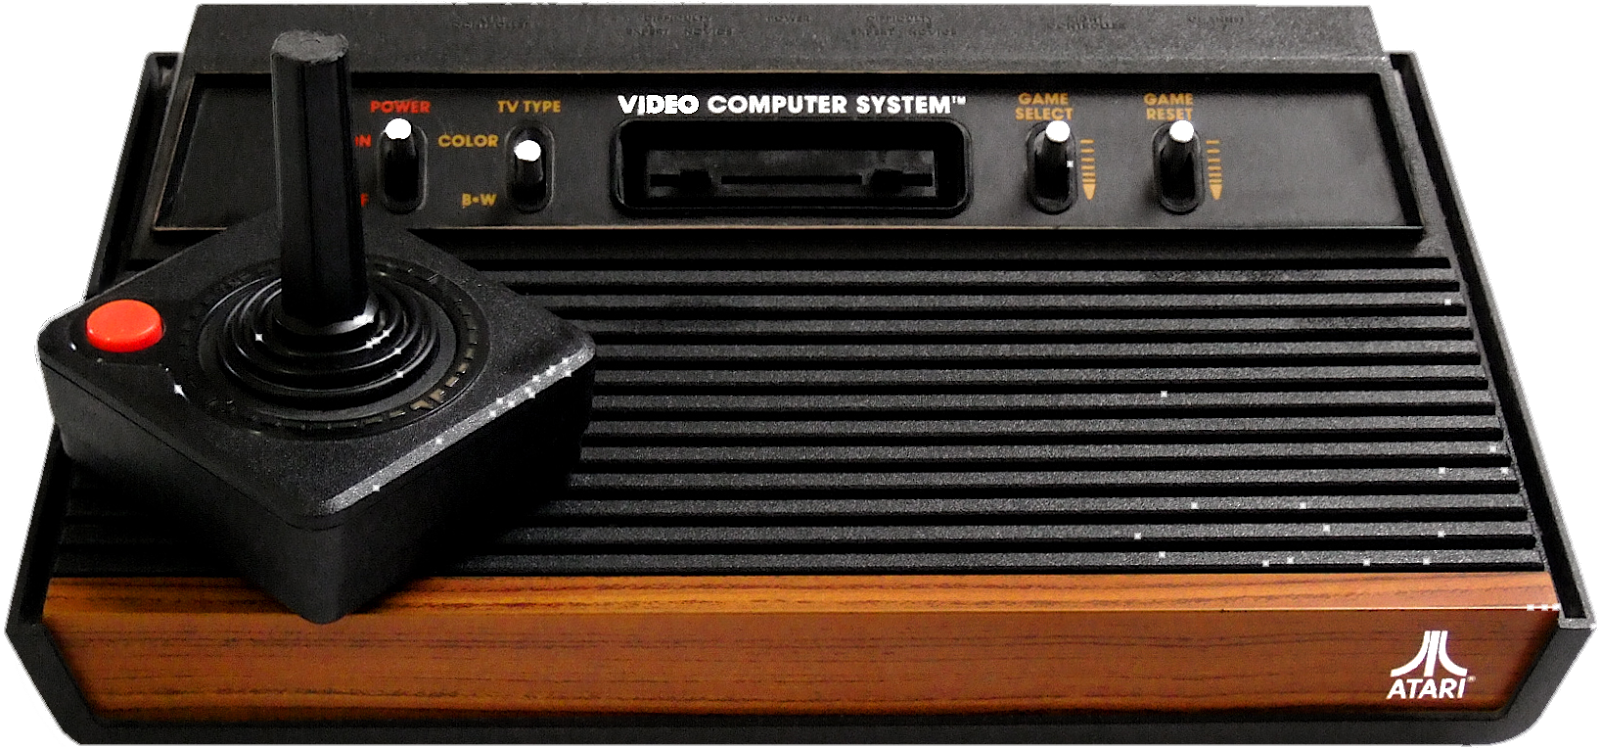
\includegraphics[width=.5\textwidth]{Atari2600}
        \end{figure}
    \end{frame}

    \begin{frame}{NES (1983)}
        \begin{multicols}{2}
            \scriptsize
            \begin{description}
                \setlength\itemsep{0em}
                \item[Processador:] MOS 6502 Customizado
                \item[Barramento:] 8 bits
                \item[Clock (CPU):] 1.79MHz (NTSC), 1.66MHz (PAL)
                \item[Clock (GPU):] 5.37MHz (NTSC), 5.33MHz (PAL)
                \item[RAM:] 2KiB + RAM Expandida (do cartucho)
                \item[ROM:] 48KB
                \item[Resolução:] 256x240
                \item[Cores:] 56 cores (paleta básica)
                \item[Cores na tela:] 25 cores por scanline (cor de fundo + 4
                    conjuntos de 3 cores de tiles + 4 conjuntos de cores por
                    sprite)
                \item[OAM:] 256 bytes
                \item[Dim. das Sprites:] 16x16 ou 24x24
                \item[Máx. Sprites na tela:] 64
                \item[Som:] 5 canais (2 square, 1 triangle, 1 ruído-branco, 1
                    modulação de código delta-pulse (DPCM) de 6 bits)
            \end{description}
        \end{multicols}
        \begin{multicols}{2}
            \begin{figure}[h!]
                \centering
                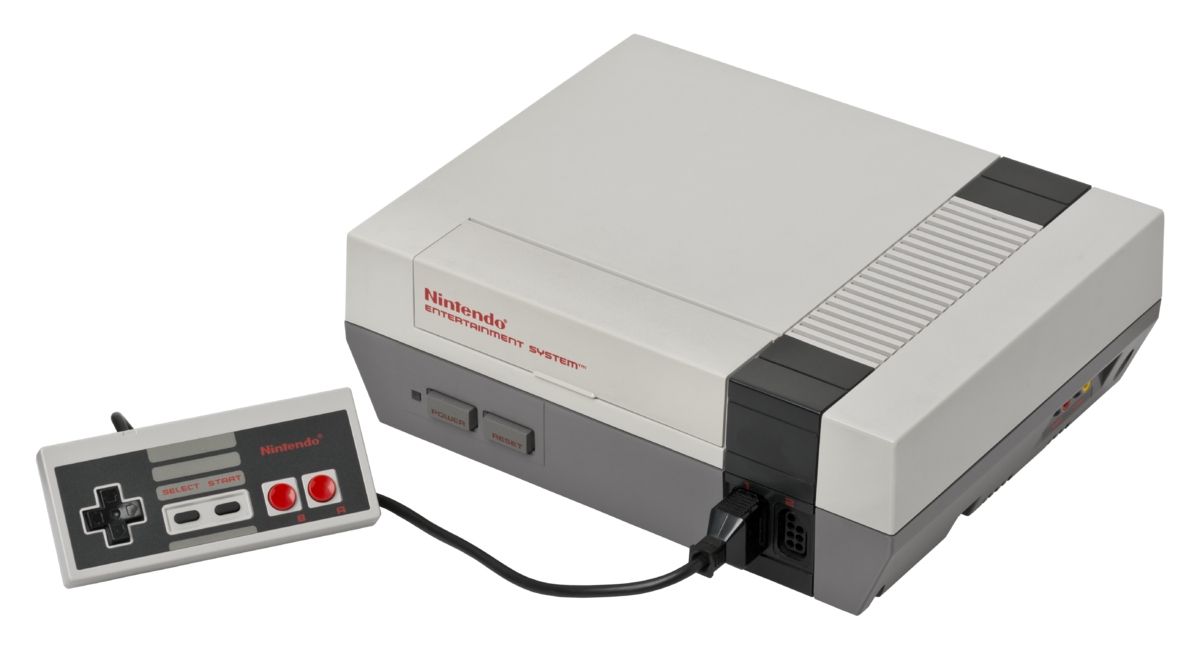
\includegraphics[height=.2\textheight]{nes}
            \end{figure}
            \begin{figure}[h!]
                \centering
                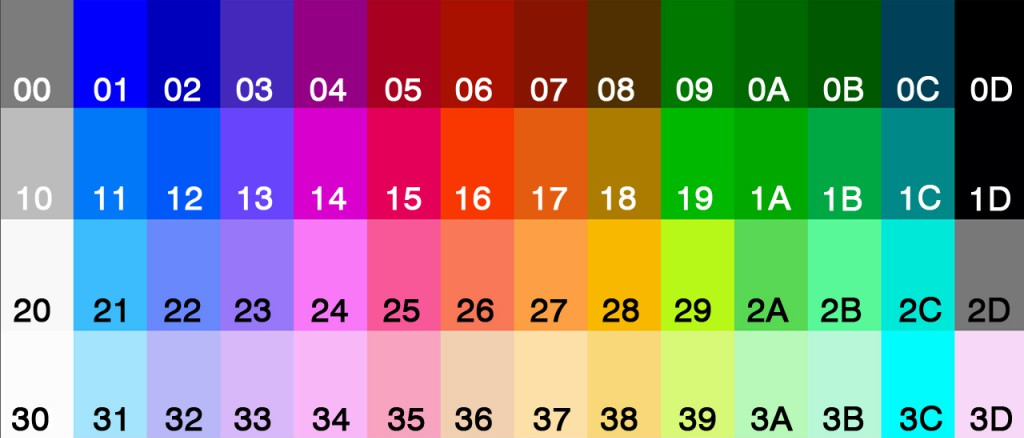
\includegraphics[height=.2\textheight]{nes_palette}
            \end{figure}
        \end{multicols}
    \end{frame}

    \begin{frame}{SNES (1990)}
        \begin{multicols}{2}
            \scriptsize
            \begin{description}
                \setlength\itemsep{0em}
                \item[Processador:] Ricoh 5A22 customizado da Nintendo
                \item[Barramento:] 16 bits
                \item[Clock (CPU):] 1.79MHz, 2.86MHz ou 3.58MHz
                \item[Clock (GPU):] Mesmo da CPU
                \item[RAM:] 128KB
                \item[VRAM:] 64KB (512 + 32 bytes de sprite, 256x15 bits de
                    paleta)
                \item[RAM (Áudio):] 64KB
                \item[Resolução:] 256x224/512x448
                \item[Cores:] 32768 (15 bits)
                \item[OAM:] 544 bytes
                \item[Dim. das sprites:] 8x8, 16x16, 32x32 e 64x64
                \item[Cores/sprite:] 16
                \item[Máx. sprites na tela:] 128 (32 na mesma linha)
                \item[Camadas de background:] 4
                \item[Som:] 8 canais (32KHz 16-bit stereo).
            \end{description}
        \end{multicols}
        \begin{multicols}{2}
            \begin{figure}[h!]
                \centering
                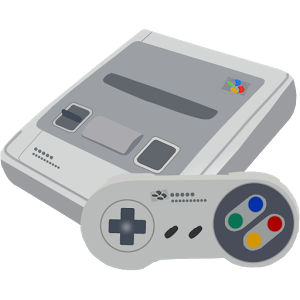
\includegraphics[height=.2\textheight]{snes}
            \end{figure}
            \begin{figure}[h!]
                \centering
                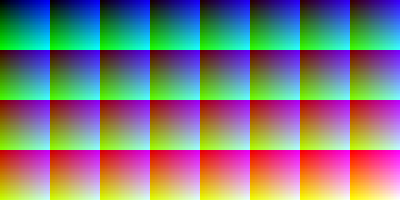
\includegraphics[height=.2\textheight]{snes_palette}
            \end{figure}
        \end{multicols}
    \end{frame}

    \begin{frame}{GameBoy (1989)}
        \begin{multicols}{2}
            \scriptsize
            \begin{description}
                \setlength\itemsep{0em}
                \item[Processador:] Sharp LR35902 Customizado
                \item[Barramento:] 8 bits
                \item[Clock (CPU):] 4.19MHz
                \item[RAM:] 8KB (podendo ser expandido para 32KB)
                \item[ROM:] 256 bytes (interno),
                    256K/512K/1M/2M/4M/8M (cartuchos)
                \item[VRAM:] 8KB (interno)
                \item[Resolução:] 160x144
                \item[Cores:] 2 bits (4 tons de \enquote{cinza})
                \item[OAM:] 160 bytes (4 bytes/sprite)
                \item[Dim. das sprites:] 8x8, 8x16
                \item[Cores/sprite:] 16
                \item[Máx. sprites na tela:] 40
                \item[Som:] 2 geradores de pulso de onda
            \end{description}
        \end{multicols}
        \begin{multicols}{2}
            \begin{figure}[h!]
                \centering
                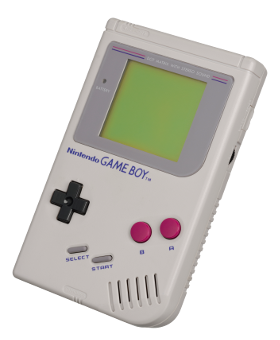
\includegraphics[height=.2\textheight]{gb}
            \end{figure}
            \begin{figure}[h!]
                \centering
                
\includegraphics[height=.2\textheight]{gb_palette}
            \end{figure}
        \end{multicols}
    \end{frame}

    \begin{frame}{GameBoy Advance (2001)}
        \begin{multicols}{2}
            \scriptsize
            \begin{description}
                \setlength\itemsep{0em}
                \item[Processador:] ARM7 TDMI com memória embarcada
                \item[Barramento:] 16 bits
                \item[Co-processador:] Z80 8-bit de 4/8MHz (para
                    compatibilidade com GB/GBC)
                \item[Clock (CPU):] 16.8MHz
                \item[Clock (GPU):] ~5.5MHz (\textbf{59.73FPS})
                \item[RAM:] 32KB (CPU)
                \item[VRAM:] 92KB (interno)
                \item[DRAM:] 256KB (externa à CPU)
                \item[Resolução:] 240x160 (3:2)
                \item[Cores:] 15-bit BGR (5 bits/canal), 512 cores (character
                    mode), 32768 cores (bitmap mode)
                \item[OAM:] 160 bytes (4 bytes/sprite)
                \item[Dim. das sprites:] 8x8, 8x16, 8x32, 16x8, 16x16, 16x32,
                    32x8, 32x16, 32x32, 32x64, 64x32, 64x64
                \item[Cores:] 256 (1 paleta para toda a tela)
                \item[Máx. sprites na tela:] 256
                \item[Som:] Dual 8-bit DAC para som Stereo (DirectSound)
            \end{description}
        \end{multicols}
        \begin{multicols}{2}
            \begin{figure}[h!]
                \centering
                
\includegraphics[height=.2\textheight]{gba}
            \end{figure}
            \begin{figure}[h!]
                \centering
                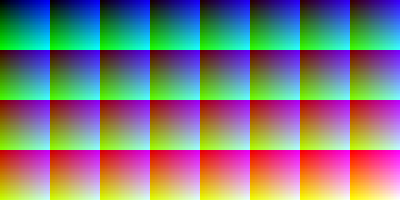
\includegraphics[height=.2\textheight]{snes_palette}
            \end{figure}
        \end{multicols}
    \end{frame}

    \begin{frame}{GameBoy Advance (2001)}
        \begin{description}
            \item[ARM7-TDMI]: ARM7 + 16-bit \underline{T}humb + JTAG
                \underline{D}ebug + fast \underline{M}ultiplier + enhanced
                \underline{I}CE.
            \item[DAC:]
                \underline{D}igital-\underline{A}nalogic-\underline{C}onverter
        \end{description}
    \end{frame}

    \section{Conhecendo a plataforma}
    \subsection{O interior do GBA}
    \begin{frame}{}
        \huge \textbf{O interior do GBA}
    \end{frame}

    \begin{frame}{Interior do GBA (frontal)}
        \begin{figure}[h!]
            \centering
            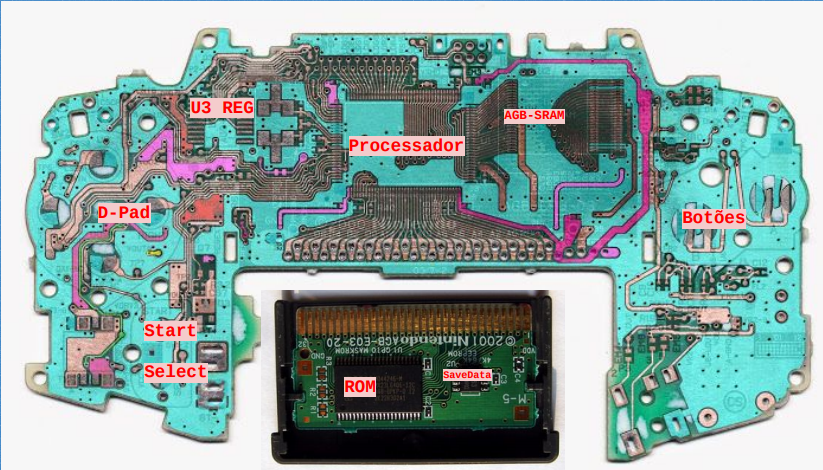
\includegraphics[width=1\textwidth,height=1\textheight,keepaspectratio]{gba_inside_front}
        \end{figure}
    \end{frame}

    \begin{frame}{Interior do GBA (frontal)}
        \begin{figure}[h!]
            \centering
            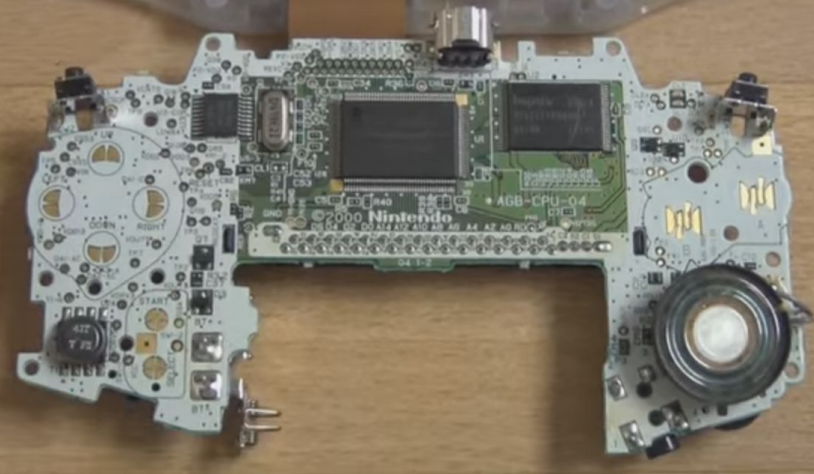
\includegraphics[width=1\textwidth,height=1\textheight,keepaspectratio]{gba_inside_front_real}
        \end{figure}
    \end{frame}

    \begin{frame}{Interior do GBA (trás)}
        \begin{figure}[h!]
            \centering
            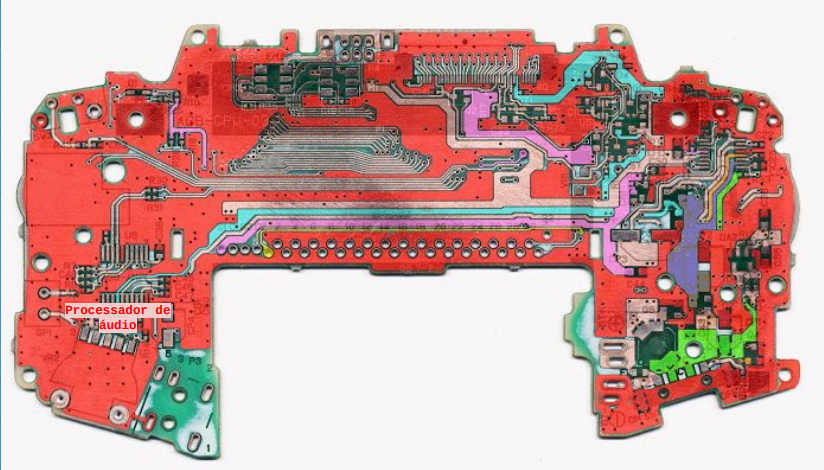
\includegraphics[width=1\textwidth,height=1\textheight,keepaspectratio]{gba_inside_back}
        \end{figure}
    \end{frame}

    \begin{frame}{Interior do GBA: Processador}
        \begin{figure}[h!]
            \centering
            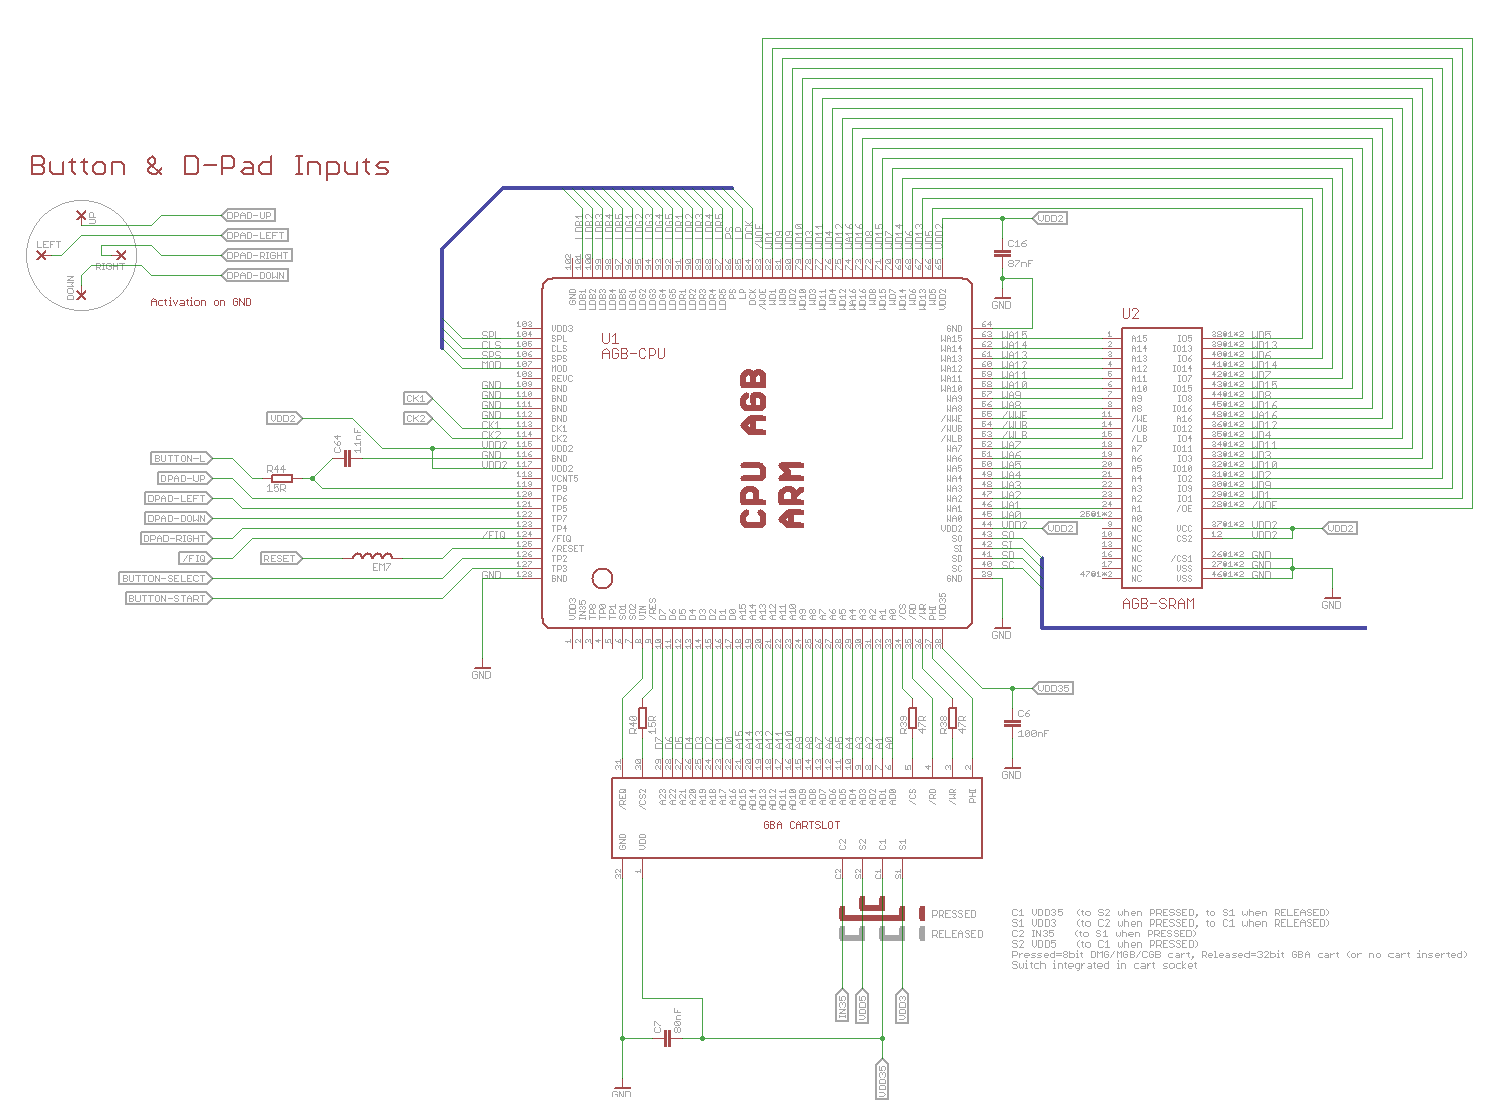
\includegraphics[width=0.95\textwidth,height=0.95\textheight,keepaspectratio]{gba_processor}
        \end{figure}
    \end{frame}

    \begin{frame}{Organização da Memória (Geral)}
        \begin{center}
            \begin{tabular}{|r|c|c|}
                \hline
                Descrição             & Início               & Fim \\\hline
                BIOS - ROM do Sistema & \texttt{0x0000:0000} & \texttt{0x0000:3FFF} \\\hline
                -                     & \texttt{0x0000:4000} & \texttt{0x01FF:FFFF} \\\hline
                WorkRAM On-Board      & \texttt{0x0200:0000} & \texttt{0x0203:FFFF} \\\hline
                -                     & \texttt{0x0200:4000} & \texttt{0x02FF:FFFF} \\\hline
                WorkRAM On-Chip       & \texttt{0x0300:0000} & \texttt{0x0300:7FFF} \\\hline
                -                     & \texttt{0x0300:8000} & \texttt{0x03FF:FFFF} \\\hline
                Registradores de I/O  & \texttt{0x0400:0000} & \texttt{0x0400:03FE} \\\hline
                -                     & \texttt{0x0400:0400} & \texttt{0x04FF:FFFF} \\\hline
            \end{tabular}
        \end{center}
    \end{frame}

\end{darkframes}
\end{document}
